\section{Results}
\label{sec:results}
We present our multi-probe constraints on the cosmological parameters of the flat $\Lambda$CDM model in Fig.~\ref{fig:cosmology-params}, showing the marginalised posterior distributions for matter fluctuation amplitude parameter, $\sigma_8$, the matter density parameter $\Omega_{\rm m}$ and the dimensionless Hubble parameter $h$, where the BOSS galaxy clustering constraints (GC: shown blue), break the $\sigma_8$-$\Omega_{\rm m}$ degeneracy in the KiDS-1000 cosmic shear constraints (CS: shown pink), resulting in tight constraints on $\sigma_8$ in the combined \tttp analysis (shown red). 
Reporting the MAP values with PJ-HPD credible intervals for the parameters that we are most sensitive to, we find 
\preliminary{\eqa{
\sigma_8 &= 0.76^{+0.021}_{-0.023} \\ \nonumber
\Omega_{\rm m} &= 0.306^{+0.011}_{-0.014} \\ \nonumber
S_8 &= 0.769^{+0.018}_{-0.015} \, .
}}
Our constraints can be compared to the marginalised posterior distributions from {\it Planck} (shown green in Fig.~\ref{fig:cosmology-params}), finding consistency between the marginalised constraints on $\Omega_{\rm m}$ and $h$, but an offset in $\sigma_8$,  which we discuss in detail in Sect.~\ref{sec:planck_comp}.

Tabulated constraints for the full set of cosmological parameters are presented in Appendix~\ref{app:parameter-constraints}, quoting our fiducial MAP with PJ-HPD credible intervals, along with the marginal posterior mode with M-HPD credible intervals. 
We note that the quoted marginal mode constraint on $S_8$ is \preliminary{$0.2\sigma$} lower than the MAP for this parameter. 
As discussed in \citet{joachimi/etal:inprep}, this marginal mode estimate is known to yield systematically low values of $S_8$ in mock data analyses, as can be seen in Fig.~\ref{fig:S8comp}, which compares the joint posterior constraints (solid) with the marginal posterior constraints (dashed).  

\begin{figure}
	\begin{center}
		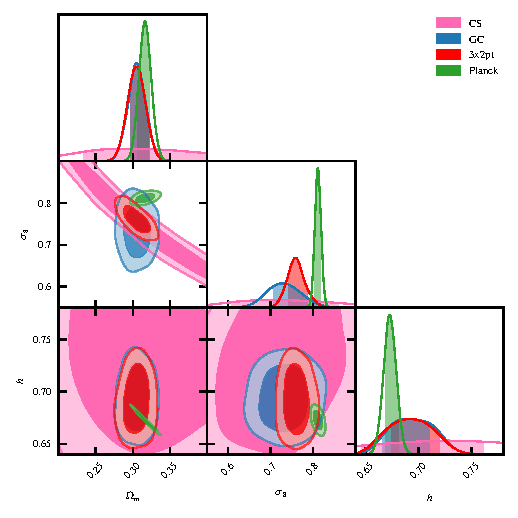
\includegraphics[width=\columnwidth]{Parameter_Plots/cosmology/omegam_sigma8_h_blind_C}
		\caption{Marginal multi-probe constraints on the flat $\Lambda$CDM cosmological model, for the matter fluctuation amplitude parameter, $\sigma_8$, the matter density parameter $\Omega_{\rm m}$, and the dimensionless Hubble parameter, $h$.  The BOSS galaxy clustering constraints (blue), can be compared to the KiDS-1000 cosmic shear constraints (pink), the combined $3\times2{\rm pt}$ analysis (red), and CMB constraints from \citet{planck/etal:2018}, (green).}
		\label{fig:cosmology-params}
	\end{center}
\end{figure}

We find good agreement between the different probe combinations and single-probe $S_8$ constraints, demonstrating internal consistency between the different cosmological probes, in Fig.~\ref{fig:S8comp}.  
As forecast by \citet{joachimi/etal:inprep}, the addition of the galaxy-galaxy lensing observable adds very little constraining power, with similar results found for the full \tttp analysis and the combined cosmic shear and clustering analysis. 
This is a result of the significant area of BOSS in comparison to KiDS-1000, and the fact that our lack of an accurate galaxy bias model on the deeply non-linear scales that weak lensing probes,
prohibits the inclusion of large sections of our galaxy-galaxy lensing data vector, shown in Fig.~\ref{fig:Pgk}.  
The addition of the galaxy-galaxy lensing does however serve to moderately tighten constraints on the amplitude of the intrinsic alignment model $A_{\rm IA}$,  as seen in Fig.~\ref{fig:cosmology-params-all}. 

Fig.~\ref{fig:S8comp} also demonstrates the good agreement between our constraints and weak lensing results from the literature, comparing to cosmic shear-only results from the Hyper Suprime-Cam Strategic Program \citep[HSC,][]{hikage/etal:2019,hamana/etal:2020}, DES \citep{troxel/etal:2018} and an earlier KiDS analysis \citep[KV450][]{hildebrandt/etal:2020}, in addition to the previous KV450-BOSS `$2\times2$pt' analysis of \citet{troester/etal:2020} and the DES Y1 \tttp analysis from \citet{abbott/etal:2018}.   We refer the reader to \citet{asgari/etal:inprep} for a discussion and comparison of different cosmic shear results.  In Sect.~\ref{sec:WL_comp} we present a more detailed comparison of our results with \tttp results in the literature.

\begin{figure}
	\begin{center}
		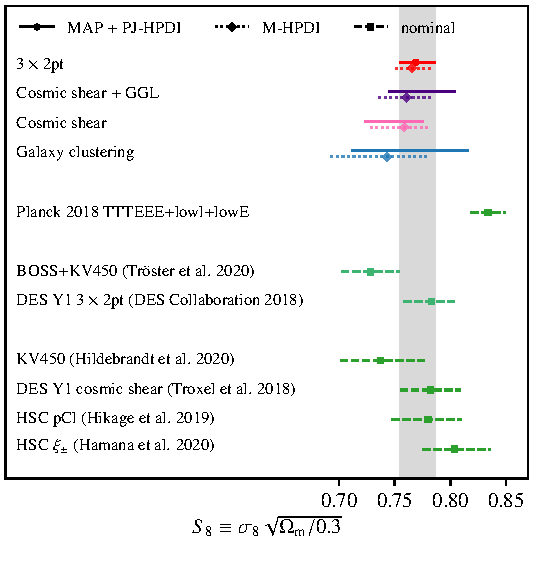
\includegraphics[width=\columnwidth]{Parameter_Plots/cosmology/S8_comparison_blindC}
		\caption{Constraints on structure growth parameter $S_{8} = \sigma_8 \sqrt{\Omega_{\rm m}/0.3}$ for different probe combinations: $3\times2$pt, cosmic shear with galaxy-galaxy lensing (GGL), and cosmic shear with galaxy clustering, along with the single probe analyses.   Our fiducial and preferred MAP with PJ-HPD credible interval (solid) can be compared to the standard, but biased, marginal posterior mode with M-HPD credible intervals (dotted).    Our results can also be compared to weak lensing measurements from the literature, which typically quote the mean of the marginal posterior mode with tail credible intervals (dashed). 
		\ch{TO DO:  Add CS+GC to this figure}
		\label{fig:S8comp}}
	\end{center}
\end{figure}

Fig.~\ref{fig:cosmology-params-all} displays the marginal posterior distributions for an extended set of cosmological parameters.  
We find that the allowed range for the linear galaxy bias,  $b_1$, in each redshift bin (lower two rows), is more than halved with the addition of the weak lensing data. 
This constraint does not arise, however, from the sensitivity of the galaxy-galaxy lensing observable to galaxy bias (shown to be relatively weak in the CS+GGL contours). 
Instead, in this analysis, it is a result of the degeneracy breaking in the $\sigma_8$-$\Omega_{\rm m}$ plane, tightening constraints on $\sigma_8$ which, for galaxy clustering, is degenerate with galaxy bias. 
The improved constraints on galaxy bias do not, however, fold through to improved constraints on $h$, which the weak lensing data adds very little information to. 

For our primary cosmological parameter, $S_8$, our constraints are uninformed by our choice of priors.    This statement cannot be made for the other $\Lambda$CDM parameters, however, as shown in Fig.~\ref{fig:cosmology-params-all}.   The most informative prior that we have introduced to our \tttp analysis is on the spectral index, $n_{\rm s}$.  As noted by \citet{troester/etal:2020}, the BOSS galaxy clustering constraints favour a low value for $n_{\rm s}$, where they find $n_{\rm s} = 0.815 \pm 0.085$. 
From the \citet{troester/etal:2020} sensitivity analysis to the adopted maximum clustering scale, we observe that this preference appears to be driven by the amplitude of the large scale clustering signal with $s > 100 \, h^{-1}\, {\rm Mpc}$.  We note that spurious excess power in this regime could plausibly arise from variations in the stellar density impacting the BOSS galaxy selection function \citep{ross/etal:2017}.  Our choice to impose a theoretically motivated informative prior for $n_{\rm s}$, as listed in Table~\ref{tab:priors}, helps to negate this potential systematic effect without degrading the overall goodness of fit to the galaxy clustering measurements.  Our prior choice is certainly no more informative than the $n_{\rm s}$ priors that are typically used in weak lensing and clustering analyses \citep[see for example][]{abbott/etal:2018}. 
We recognise, however, that this well-motivated prior choice acts to improve the BOSS-only error on $\Omega_{\rm m}$ by roughly a third, and decrease the BOSS-only best-fitting value for $\Omega_{\rm m}$ and $h$ by $\sim 0.5\sigma$.  With $<10\%$ differences on the constraints on $S_8$ and $h$, however, and only a $\sim 0.1\sigma$ difference in the BOSS-only best-fitting value for $S_8$, which is consistent with the typical variation between different {\sc Multinest} analyses, we conclude that our prior choice does not impact on our primary $S_8$ constraints.   With the informative or uninformative $n_{\rm s}$ prior, our constraints on $h$ remain consistent with the Hubble parameter constraints from both \citet{planck/etal:2018} and \citet{riess/etal:2019}.

\begin{figure*}
	\begin{center}
		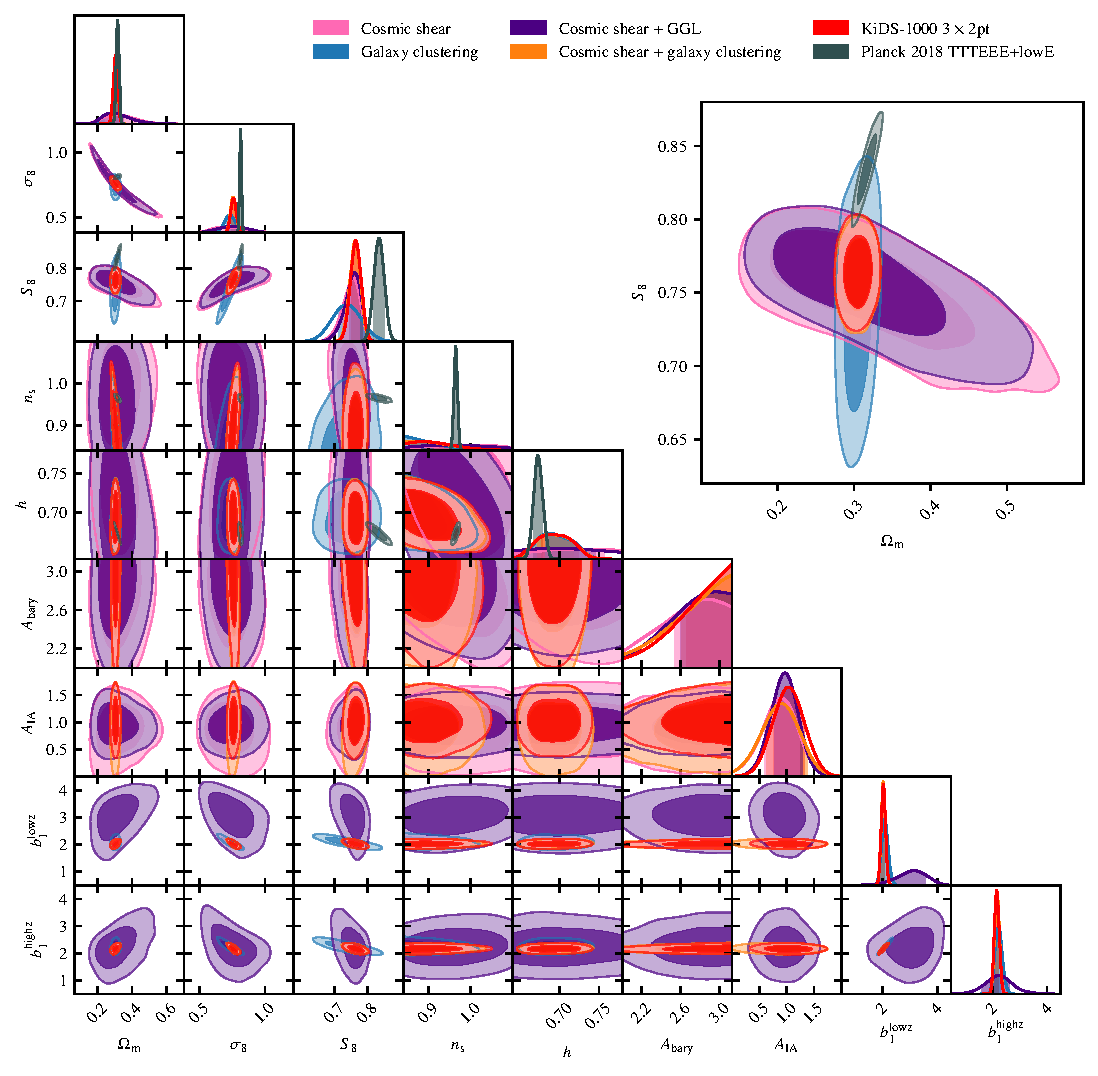
\includegraphics[width=\textwidth]{Parameter_Plots/cosmology/omegam_sigma8_s8_ns_h_a_baryon_a_ia_b1l_b1h_blind_C}
		\caption{Marginalised posterior distributions for an extended set of cosmological parameters covering the matter density parameter $\Omega_{\rm m}$, the matter fluctuation amplitude parameter, $\sigma_8$, the structure growth parameter $S_8$, the spectral index $n_{\rm s}$, the dimensionless Hubble parameter, $h$, the baryon feedback amplitude parameter, $A_{\rm baryon}$, the intrinsic alignment amplitude, $A_{\rm IA}$, and the linear bias parameters for the low and high BOSS redshift bins, $b_1$.   The KiDS-1000 cosmic shear results (pink), can be compared to the BOSS galaxy clustering results (blue), the combination of cosmic shear with BOSS and 2dFLenS galaxy-galaxy lensing (GGL, purple), and the full $3\times2$pt (red).   For parameters constrained by the CMB, we also include constraints from \citet{planck/etal:2018} (green).}
		\label{fig:cosmology-params-all}
	\end{center}
\end{figure*}


Fig.~\ref{fig:S8comp_sensitivity} illustrates the results of a series of sensitivity tests, where we explore how our \tttp constraints on $S_8$ change when: 
we ignore the impact of baryon feedback (the `No baryon' case), fixing $A_{\rm baryon}=3.13$, corresponding to the non-linear matter power spectrum for a dark-matter only cosmology; 
we limit the analysis to a linear galaxy bias model, setting all higher-order bias terms in Eq. (\ref{eq:pgg}) to zero, as well as restricting the redshift-space distortion model to a Gaussian velocity distribution; 
and when we remove individual tomographic bins from our weak lensing observables. 
The only outlier in this series of tests is the linear-bias model, which highlights the importance of accurate non-linear galaxy bias modelling in \tttp analyses. 
This series of tests complements the more detailed KiDS-1000 internal consistency analysis of \citet{asgari/etal:inprep}, and is dissected in Appendix~\ref{app:sensitivity}.

\begin{figure}
	\begin{center}
		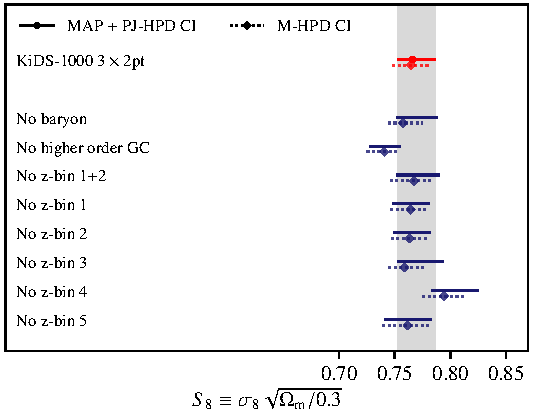
\includegraphics[width=\columnwidth]{Parameter_Plots/systematics/S8_comparison_blindC}
		\caption{\tttp constraints on $S_8$ for a series of sensitivity tests; when we ignore the impact of baryon feedback (the `No baryon' case), limit the analysis to a linear galaxy bias model (the `No higher order bias' case), and remove individual tomographic bins from our weak lensing observables.    
		\TT{Note that only the 3x2pt chain has the BOSS CosmoSIS-interface bug fixed, hence the overall offset - this will be fixed with the new runs!}
		\label{fig:S8comp_sensitivity}}
	\end{center}
\end{figure}

Table~\ref{tab:goodness-of-fit} records the goodness of fit for each component in our \tttp analysis, given the MAP cosmological parameters.  For our \tttp analysis we have implemented an optimised MAP-finder (see Sect.~\ref{sec:KCAP}), in order to estimate the minimum $\chi^2$.  For all other analyses we only report the noisy MAP estimate from {\sc Multinest}, providing an upper limit for the goodness of fit.  
The effective number of degrees of freedom (DoF) are calculated using the estimator described in section 6.3 of \citet{joachimi/etal:inprep}, which accounts for the impact of priors and non-linear dependencies between the parameters.  
The goodness of fit is excellent for the BOSS galaxy clustering.  For all other cases, the goodness of fit is certainly acceptable\footnote{We define acceptable as $p \geq 0.001$, which corresponds to less than a $\sim 3\sigma$ event.   \citet{abbott/etal:2018} define acceptable as $\chi^2/{\rm DoF} < 1.4$.  We meet both these requirements.}.
We note that the cosmic shear analysis of \citet{asgari/etal:inprep}, where a different choice in the cosmic shear two-point statistic results in an excellent goodness of fit, shows no significant changes in the inferred cosmological parameters.    As such, we could be subject to an unlucky noise fluctuation that particularly impacts the band power estimator in Eq. (\ref{eq:cl_cosmicshear}).  Cautiously inspecting Fig.~\ref{fig:Pkk}, as `$\chi$-by-eye' is particularly dangerous with correlated data points, we nevertheless note a handful of outlying points, for example the low $\ell$-scales in the fifth tomographic bin.   We also note that \citet{giblin/etal:inprep} document a significant but low-level PSF residual systematic in the KiDS-1000 fourth and fifth tomographic bins that was shown to reduce the overall goodness of fit in a cosmic shear analysis, but not bias the recovered cosmological parameters \citep[see also the discussion in][]{amara/refregier:2008}.  Future work to remove these low-level residual distortions is therefore expected to further improve the goodness of fit.

\begin{table}
	\begin{center}
		\caption{The goodness of fit of the flat $\Lambda$CDM cosmological model to each of the single and joint probe combinations with cosmic shear, galaxy clustering (GC) and galaxy-galaxy lensing (GGL).}
		\label{tab:goodness-of-fit}
\begin{tabular}{lrcl}
    \toprule
    Probe             & $\chi^2$       & DoF       & $p$-value   \\
    \midrule
	Cosmic shear     & $< 152.7$ & $120-\preliminary{3.0}$ & 0.015 \\
	Galaxy clustering (GC) & $< 169.5$ & $168-\preliminary{10.6}$ & 0.241 \\
	Cosmic shear + GGL & $< 180.6$ & $142-\preliminary{7.3}$ & 0.005 \\
	Cosmic shear + GC & $< 323.0$ & $288-\preliminary{11.9}$ & 0.028 \\
	KiDS-1000 $3\times2$pt & $< 352.9$ & $310-\preliminary{12.5}$ & 0.015 \\

    \bottomrule
\end{tabular}
	\end{center}
	\tablefoot{We list the minimum $\chi^2$ value, the effective number of degrees of freedom (DoF) and the corresponding $p$-value which describes the probability of producing measurements that are more extreme than the data, assuming the cosmological model is correct.   The DoF is presented as the difference between the total number of data points and the effective number of free parameters, accounting for the impact of priors and non-linear dependencies between the parameters.}
\end{table}

\subsection{Comparison with weak lensing surveys}
\label{sec:WL_comp}
Our results are consistent with weak lensing constraints in the literature.   We limit our discussion in this section to published \tttp analyses, referring the reader to \citet{asgari/etal:inprep} who discuss how the KiDS-1000 cosmic shear results compare with other weak lensing surveys.   We note that direct comparisons of cosmological parameters should be approached with some caution, as the priors adopted by different surveys and analyses are often informative \citep[see section 6.1 in][]{joachimi/etal:inprep}.   Homogenising priors for cosmic shear analyses, for example, has been shown to lead to different conclusions when assessing inter-survey consistency \citep{chang/etal:2019, joudaki/etal:2020, asgari/etal:2020_KD}.   

\begin{figure}
	\begin{center}
		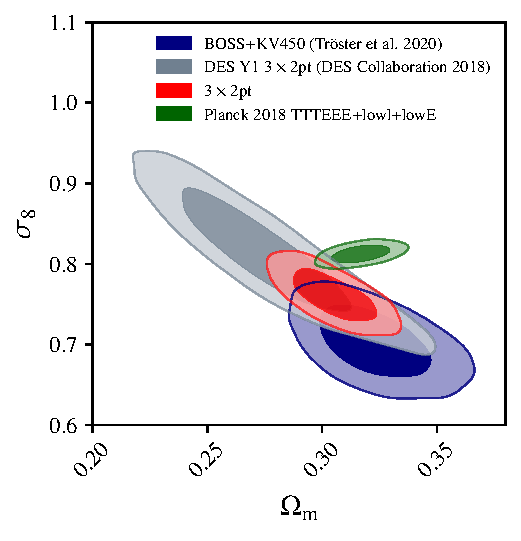
\includegraphics[width=\columnwidth]{Parameter_Plots/cosmology/omegam_sigma8_survey_comparison}
		\caption{Marginalised posterior distribution in the $\sigma_8$-$\Omega_{\rm m}$ plane, comparing the \tttp analyses from KiDS-1000 and DES Y1 \citep{abbott/etal:2018} with the CMB constraints from \citet{planck/etal:2018}.   The KiDS-1000-BOSS result can also be compared to our previous KV450-BOSS analysis from \citet{troester/etal:2020}. 
		\label{fig:DES_KiDS_comp}}
	\end{center}
\end{figure}


\citet{abbott/etal:2018} present the first year \tttp DES analysis (DES Y1), finding $S_8=0.773^{+0.026}_{-0.020}$, where they report the marginal posterior maximum and the tail credible intervals.  
This is in excellent agreement with our equivalent result, differing by $0.2\sigma$, with the KiDS-1000-BOSS error being 30\% tighter than the DES Y1 results.  The inclusion of BOSS to our \tttp analysis results in tight constraints on $\Omega_{\rm m}$.  
This leads to joint KiDS-1000-BOSS constraints on $\sigma_8=0.760^{+0.021}_{-0.023}$ that are more than twice as constraining compared to DES Y1 which finds $\sigma_8=0.817^{+0.045}_{-0.056}$, as shown in Fig.~\ref{fig:DES_KiDS_comp}. 
This comparison serves to highlight the additional power that can be extracted through the combination of spectroscopic and photometric surveys,  and the promising future for the planned overlap between the Dark Energy Spectroscopic Instrument survey \citep{DESI/etal:2016} and the 4-metre Multi-Object Spectroscopic Telescope \citep[4MOST,][]{guiglion/etal:2019},
with Euclid and the Vera C. Rubin Legacy Survey of Space and Time \citep{laureijs/etal:2011,lsst/etal:2009}, in addition to the nearer-term $\approx\!1400\,\mathrm{deg}^{2}$ of overlap between BOSS and the Hyper Suprime-Cam Strategic Program \citep[HSC,][]{aihara/etal:2019}. 

\citet{vanuitert/etal:2018} and \citet{joudaki/etal:2018} present \tttp analyses for the second KiDS release (KiDS-450), finding, respectively, $S_8 = 0.800_{-0.027}^{+0.029}$ (KiDS with GAMA) and $S_8 = 0.742 \pm 0.035$ (KiDS with BOSS and 2dFLenS limited to the overlap region). 
Both results are consistent with our KiDS-1000 results, noting that the increase in our $S_8$ constraining power, by a factor of $\approx\! 2$ in this analysis, is driven by increases in both the KiDS survey area, and the BOSS survey area.  

The impact of doubling the KiDS area can be seen by comparing to \citet{troester/etal:2020}, in Fig.~\ref{fig:DES_KiDS_comp}, who present a joint cosmic shear and galaxy clustering analysis of the KV450 KiDS release with the full BOSS area, finding $S_8 = 0.728 \pm 0.026$.   The $\approx\!40\%$ improvement in constraining power is consistent with expectations from the increased survey area, but a straightforward area-scaling comparison is inappropriate given that KiDS-1000 features improvements in the accuracy of the shear and photometric redshift calibrations, albeit at the expense of a decrease in the effective number density \citep[see][for details]{giblin/etal:inprep}.  
The offset of $1.3\sigma$ in $S_8$ between the KiDS-1000-BOSS and KV450-BOSS $S_8$ constraints reflects a number of differences in the analyses.  First, as the \tttp $S_8$ constraints are primarily driven by KiDS (see Fig.~\ref{fig:cosmology-params-all}), we expect a reasonable statistical fluctuation in this parameter given the increase in the KiDS survey area by a factor of two, even though the BOSS area remains fixed.   In contrast, BOSS primarily constrains $\Omega_{\rm m}$ which is impacted by the choice of prior on $n_{\rm s}$.  The wider $n_{\rm s}$ prior adopted in \citet{troester/etal:2020}, favours a slightly higher but less well-constrained value for $\Omega_{\rm m}$, leading to a slightly lower but less well-constrained value for $\sigma_8$, when combined with cosmic shear.   If we had also chosen an uninformative prior on $n_{\rm s}$ for our KiDS-1000-BOSS analysis, a decision that we now cannot revise post unblinding, this would have likely served to further exacerbate any tension with the {\it Planck} CMB constraints.   



\subsection{Comparison with {\it Planck}}
\label{sec:planck_comp}
In our KiDS-1000-BOSS \tttp analysis, we find good agreement with {\it Planck} for the matter density parameter, $\Omega_{\rm m}$, and the Hubble parameter, $h$, (see Fig.~\ref{fig:cosmology-params}).
The amplitude of matter fluctuations, $\sigma_8$, that we infer from the clustering of galaxies within, and lensing by, the large-scale structure of the low-redshift Universe is lower than that inferred by {\it Planck}\footnote{A recent independent Atacama Cosmology Telescope CMB analysis reports $S_8=0.830 \pm 0.043$, in agreement with the {\it Planck} constraint of $S_8=0.834 \pm 0.016$ \citep[ACT,][]{aiola/etal:2020}.   Our results are fully consistent with the ACT CMB analysis, reflecting the larger uncertainty in the ACT constraints.} from the CMB, however. 

To quantify this discrepancy in the amplitude of matter fluctuations we concentrate on the parameter $S_{8} = \sigma_8 \sqrt{\Omega_{\rm m}/0.3}$ as it is tightly constrained and only exhibits negligible degeneracies, if at all, with the other cosmological parameters, $\Omega_{\rm m}$, $h$, and $n_{\rm s}$, as illustrated in Fig.~\ref{fig:cosmology-params-all}. 
%
The difference in the marginal posterior of $S_{8}$ between our \tttp analysis and the {\it Planck} \software{plik\_lite\_TTTEEE}+\software{lowl}+\software{lowE} likelihood, measured as the difference in the means divided by the standard deviations added in quadrature, is \kpoff.

Our results thus continue the trend of low-redshift probes preferring low amplitudes of matter fluctuations \citep{heymans/etal:2013, alam/etal:2017, abbott/etal:2018, hikage/etal:2019, wright/etal:2020b,DESclusters/etal:2020}. 
In these cases the reported low $S_8$, or $\sigma_8$, constraints are formally statistically consistent with {\it Planck}, and well below the detection of any anomalies at the $5\sigma$-level. 
Considering, however, the $\sim 3\sigma$ difference that we have reported, and the overall trend amongst independent probes, we would argue that we have now reached an uncomfortable point when it comes to regarding the $S_8$ offset as a simple statistical fluke.

\citet{Sanchez2020} pointed out that comparing $S_{8}$ between different experiments can be misleading due to the implicit dependence of $\sigma_{8}$ on $h$ through the $8\,h^{-1}{\rm Mpc}$ radius of the sphere within which the matter fluctuations are measured. 
A high value of $h$ would result in $\sigma_{8}$ measuring fluctuations within a smaller physical radius and thus inferring higher fluctuations. 
We thus also consider $S_{12} = \sigma_{12}\left(\omega_{\rm m}/0.14\right)^{0.4}$ \citep{Sanchez2020}, where $\sigma_{12}^{2}$ is the variance of the linear matter field at redshift zero in spheres of radius $12\,\mathrm{Mpc}$.
We find $S_{12} = 0.754^{+0.015}_{-0.018}$, with the value inferred by {\it Planck} being $S_{12} = 0.817_{-0.015}^{+0.011}
$, a discrepancy of $3.0\sigma$. 
This is in agreement with the results for $S_{8}$. 
Considering that our \tttp constraints on $h$ agree with those of {\it Planck}, and our $S_{8}$ constraints show no degeneracy with $h$, this is not surprising.

In light of the large parameter spaces that are being considered, focussing on a single parameter paints a simplistic picture on the agreement or disagreement between these probes, however. 
On a fundamental level, the question we wish to answer is whether a single model of the Universe can describe both the CMB as well as the low-redshift large-scale structure of the Universe.
Within our Bayesian inference framework, the Bayes factor provides a natural approach to model selection. 
The two models under consideration are 
\begin{description}
	\item[$\mathrm{M}_1$:] Both our \tttp data and {\it Planck}'s measurements of the CMB are described by a single flat \LCDM cosmology.
	\item[$\mathrm{M}_2$:] The two data sets are described by different cosmologies for the low- and high- redshift Universe, respectively.
\end{description}
The Bayes factor is then
\be
\label{equ:bayes-factor}
	R = \frac{P(\vec d | \mathrm{M}_1)P(\mathrm{M}_1)}{P(\vec d | \mathrm{M}_2)P(\mathrm{M}_2)} \ ,
\ee
where $P(\vec d | \mathrm{M}_1)$ is the probability of the data $\vec d$ under model $\mathrm{M}_1$ -- the Bayesian evidence. 
We assume the model priors $P(\mathrm{M}_1)$ and $P(\mathrm{M}_2)$ to be equal, that is, we make no a-priori assumption on the likelihood of $\mathrm{M}_1$ or $\mathrm{M}_2$. 
We use \software{anesthetic}\footnote{\url{https://github.com/williamjameshandley/anesthetic}}\citep{anesthetic} to compute $R$ and find $\log R=3.1\pm0.3$, which can be interpreted as odds of $23\pm6$ in favour of model $\mathrm{M}_1$, i.e., consistency between our \tttp measurement and {\it Planck}. 

\citet{handley/lemos:2019} discuss the dependence of $R$ on the parameter priors and propose a statistic $S$ -- called `suspiciousness' -- based on the Bayes factor but hardened against prior-dependences. 
They define 
\be
\label{equ:suspiciousness}
 \log S = \log R - \log I \,.
\ee
Here $\log R$ is the logarithm of the Bayes factor in Eq.~\eqref{equ:bayes-factor}:
\be
	\log R = \log Z_{{\rm 3\times2pt+}{\it Planck}}- \log Z_{\rm 3\times2pt} - \log Z_{\it Planck} \,,
\ee 
with the evidence $Z_{i}$ given by
\be
	Z = \int \mathcal{L}\, \pi\diff\vec\theta \,,
\ee
the integral of the likelihood $\mathcal{L}$ and prior $\pi$ over the parameters $\vec\theta$. 
The information ration $I$ in Eq.~\eqref{equ:suspiciousness} is defined as
\be
 \log I = \mathcal{D}_{\rm 3\times2pt} + \mathcal{D}_{\it Planck}  - \mathcal{D}_{{\rm 3\times2pt+}{\it Planck}} \,,
\ee
with $\mathcal{D}_{i}$ being the Kullback-Leibler divergence between the posterior $P$ and prior for probe $i$:
\begin{splitequation}
	\mathcal{D} &= \int P \log \frac{P}{\pi}\diff\vec\theta = \int P \log\mathcal{L}\, \diff\vec\theta - \log Z \\
	&= \langle\log\mathcal{L}\rangle_{P} - \log Z \,.
\end{splitequation}
The second equality follows from Bayes theorem: $P = \frac{\mathcal{L}\pi}{Z}$. 
Using this definition of $\mathcal{D}$ allows us to rephrase the suspiciousness solely in terms of the expectation values of the log-likelihoods:
\begin{splitequation}
	\log S &= \langle\log\mathcal{L}_{{\rm 3\times2pt+}{\it Planck}}\rangle_{P_{{\rm 3\times2pt+}{\it Planck}}} - \langle\log\mathcal{L}_{\rm 3\times2pt}\rangle_{P_{\rm 3\times2pt}} \\
	&\quad- \langle\log\mathcal{L}_{\it Planck}\rangle_{P_{\it Planck}} \,.
\end{splitequation}
We find $\log S=-2.0\pm0.1$. 
For Gaussian posteriors, the quantity $d-2\log S$ is distributed as $\chi^2_{d}$, where $d=d_{\rm 3\times2pt} + d_{\it Planck} - d_{{\rm 3\times2pt+}{\it Planck}}$ is the difference in the Bayesian model dimensionalities.
This allows us to assign a probability of the observed suspiciousness under the assumption that the two data sets are in concordance. 
We calculate $d$ following \citet{handley/lemos:2019} from the variances of the log-likelihoods. 
Other estimates of the Bayesian model dimensionality, such as those introduced in \citet{Raveri2019} yield very similar results. 
We calculate $d=3.3\pm0.7$ and therefore conclude that the probability of observing our measured suspiciousness statistic is $0.08\pm0.2$, or $1.8\pm0.1\,\sigma$. 

\citet{Raveri2019} introduce a number of metrics to quantify the consistency of data sets of which we consider two: $Q_{\rm DMAP}$ and $Q_{\rm UDM}$. 
The first,
\be
	Q_{\rm DMAP} =  2\log\mathcal{L}(\vec\theta^{\rm MAP}_{\rm 3\times2pt}) + 2\log\mathcal{L}(\vec\theta^{\rm MAP}_{\it Planck}) - 2\log\mathcal{L}(\vec\theta^{\rm MAP}_{{\rm 3\times2pt+}{\it Planck}}) \,,
\ee
is given by the differences of the log-likelihoods $\log\mathcal{L}(\vec\theta^{\rm MAP}_{i})$ at the MAP of the respective posteriors. 
It quantifies how the goodness-of-fit changes when the two data sets are combined. 
For Gaussian posteriors, the sampling distribution of $Q_{\rm DMAP}$ is $\chi^{2}$ with $d_{\rm 3\times2pt} + d_{\it Planck} - d_{{\rm 3\times2pt+}{\it Planck}}$ degrees of freedom. 
Here we follow \citet{Raveri2019} and calculate the model dimensionalities by $d_{i} = N - \mathrm{tr}[\mathcal{C}_{\pi}^{-1}\mathcal{C}_{P}]$, where $N$ is the total number of varied parameters, $\mathcal{C}_{\pi}$ is the prior parameter covariance, and $\mathcal{C}_{P}$ is the posterior parameter covariance. 
Using the variance of the log-likelihoods, as was done for the suspiciousness, yields consistent results.
We find \preliminary{$Q_{\rm DMAP} = 11.3$}, with $d=3.6$, corresponding to a probability of \preliminary{0.016, or $2.4\, \sigma$}. 
As an interesting aside, the quantity $Q_{\rm DMAP} + 4\log S$ corresponds to the twice the deviance information criterion ratio introduced in \citet{Joudaki2017}.

The second metric in \citet{Raveri2019} that we consider is $Q_{\rm UDM}$, which generalises the notion of parameter differences between posteriors to multiple dimensions. 
The metric is defined between the posterior of one data set and the posterior of the combined data sets:
\be
\label{equ:qudm}
	Q_{\rm UDM} = \Delta\overline{\vec\theta}^{T}(\mathcal{C}_{\it Planck} - \mathcal{C}_{{\rm 3\times2pt+}{\it Planck}})^{-1}\Delta\overline{\vec\theta} \,,
\ee
where $\Delta\overline{\vec\theta} = \bar{\vec\theta}_{\it Planck} - \overline{\vec\theta}_{{\rm 3\times2pt+}{\it Planck}}$ is the shift in the mean of the shared parameters, and $\mathcal{C}_{\it Planck}$ and $\mathcal{C}_{{\rm 3\times2pt+}{\it Planck}}$ are the posterior parameter covariances for {\it Planck} and \tttp+{\it Planck}, respectively. 
The estimator Eq.~\eqref{equ:qudm} is asymmetric in the first data set if the posteriors are non-Gaussian. 
In this case, the data set with the more Gaussian posterior should be used, which in our case is {\it Planck}. 
We use \software{tensiometer}\footnote{\url{https://github.com/mraveri/tensiometer}} to compute $Q_{\rm UDM}$ and its associated number of degrees of freedom. 
We find $Q_{\rm UDM} = 7.7$ with $d = 3$. The sampling distribution is approximated by $\chi^{2}_{d}$, such that the probability of the observed value of $Q_{\rm UDM} $ is $0.054$, or $1.9\,\sigma$. 

The different metrics to assess the consistency of our \tttp analysis with {\it Planck} are summarised in Table~\ref{tab:tension}.

\begin{table}
	\begin{center}
		\caption{Estimators of the consistency between our fiducial \tttp analysis and the \citet{planck/etal:2018} TTTEEE+lowE results. 
		The considered estimators are 1) the differences between the means in $S_{8}$, divided by the standard deviations added in quadrature 2) the Bayes ratio $R$ between a model that assumes a single cosmology for both our \tttp and the {\it Planck} data, and a model that uses separate cosmologies for the two data sets 3) the logarithm $\log R$ of the Bayes ratio 4) the suspiciousness $\log S$ \citep{handley/lemos:2019} 5),6) the concordance/discordance estimators $Q_{\rm DMAP}$ and $Q_{\rm UDM}$ \citep{Raveri2019}. 
		The fist column lists the estimator, the second column the measured value, while third and fourth columns quantify the probability of the measured value under the assumption that the two data sets are consistent.}
		\label{tab:tension}
\begin{tabular}{lccc}
    \toprule
    Estimator             & Value &PTE   & PTE [$\sigma$]\\
    \midrule
	$\frac{|\bar{S_{8}}^{\rm 3\times2pt}-\bar{S_{8}}^{\it Planck}|}{\sqrt{\mathrm{Var}[S_{8}^{\rm 3\times2pt}] + \mathrm{Var}[S_{8}^{\it Planck}]}}$     & -- & 0.001 & \kpoff  \\
	$R$     & \kR & -- & -- \\
	$\log R$    &  \klogR& -- & --\\
	$\log S$    & \klogS & \klogSPTE &\klogSPTEsigma \\
	$Q_{\rm DMAP}$    & \preliminary{$11.3$} & \preliminary{0.016} & \preliminary{$2.4\, \sigma$} \\
	$Q_{\rm UDM}$    & 7.7 & $0.054$  &$1.9\,\sigma$ \\
    \bottomrule
\end{tabular}
	\end{center}
\end{table}
















